\section{稳定曲线的形变}
\label{sec:deformations-stable-curves}
\setcounter{equation}{14}

我们先描述复结构空间 $\mathcal J_\Sigma$ 的无穷小形变空间，并为
德利涅--芒福德空间 $\overline{\mathcal M}_{g,m}$ 给出坐标图册。然后从最低维层开始，逐层归纳地构造
$\overline{\mathcal M}_{g,m}$ 的图册。最低维层中的每个元素都是若干个亏格为零、恰有三个特殊点（标记点或奇点）的曲面的并。
回忆在光滑曲面 $\Sigma$ 上，每个殆复结构的挠率都为零，因而可积。所以我们可以把复结构等同于相伴的殆复结构，并在微分几何的背景下描述
$\overline{\mathcal M}_{g,m}$。类似思路的论述可参见 (RS06)。

\subsection{复结构的形变}
\label{subsec:deformations-complex-structures}

殆复结构 $j:T\Sigma\to T\Sigma$ 是满足每一点上 $j^2=-id$ 的自同态。以 $\mathcal J_\Sigma$ 表示殆复结构的集合。
群 $\Diff(\Sigma)$ 通过推前作用于 $\mathcal J_\Sigma$：
\[
 (\phi,j)\in\Diff(\Sigma)\times\mathcal J_\Sigma
 \longmapsto \phi_*j\in\mathcal J_\Sigma,
 \qquad \phi_*j=d\phi\circ j\circ d\phi^{-1}.
\]
记
\[
 \mathcal M_g:=\mathcal J_\Sigma/\Diff(\Sigma).
\]
复化切空间分解为
\[
 T_{\mathbb C}\Sigma=T^{(1,0)}\Sigma\oplus T^{(0,1)}\Sigma,
 \qquad \overline{T^{(0,1)}\Sigma}=T^{(1,0)}\Sigma.
\]
反过来，若复子空间 $H\subset T_{\mathbb C}\Sigma$ 满足
\begin{equation}
 T_{\mathbb C}\Sigma=H\oplus\overline H,
 \label{eq:complex-splitting-deformation}
\end{equation}
便可令 $H,\overline H$ 分别为特征值 $i,-i$ 的特征空间，从而在 $T\Sigma$ 上得到殆复结构 $j$。这里把实切丛嵌入为共轭不动点集
\[
 T\Sigma\cong\left\{\frac{\xi+\overline\xi}{2}\in T_{\mathbb C}\Sigma\mid \xi\in H\right\},
\]
并定义
\[
 j_H\left(\frac{\xi+\overline\xi}{2}\right):=
 \frac{i\xi-i\overline\xi}{2}.
\]
由于 $j_H^2=-id$，分裂\eqref{eq:complex-splitting-deformation}与殆复结构等价。记 $\Pi:T_{\mathbb C}\Sigma\to T_{\mathbb C}\Sigma$ 为像为 $T^{(1,0)}\Sigma$、核为 $T^{(0,1)}\Sigma$ 的幂等算子。

现在通过考察幂等算子 $\Pi$ 的形变来研究 $\Sigma$ 上复结构的形变。固定复结构 $j$。邻近复结构 $j'$ 所对应的子空间由
\[
 \overline H=\operatorname{Graph}B,
 \qquad B\in\Gamma\!\left(\operatorname{Hom}_{\mathbb C}
 (T^{(0,1)}\Sigma,T^{(1,0)}\Sigma)\right)
 =\Omega^{(0,1)}(T^{(1,0)}\Sigma)
\]
决定，并在 $j'=j$ 时有 $B=0$。反之，范数充分小的任意 $B$ 都决定这样的 $j'$。因此复结构空间是以仿射空间
$\Omega^{(0,1)}(T^{(1,0)}\Sigma)$ 为模型的无穷维流形。（\emph{复几何中常把它简记为 $\Omega^{(0,1)}(T\Sigma)$；为避免混淆，本书保留显式的 $T^{(1,0)}\Sigma$}。）

外微分可写为 $d=\partial+\overline\partial$；在函数上
\[
 \partial=\pi^{(1,0)}\circ d=\frac{d-\sqrt{-1}\,jd}{2},
 \qquad
 \overline\partial=\pi^{(0,1)}\circ d=\frac{d+\sqrt{-1}\,jd}{2}.
\]
由 $d^2=0$，有
\[
 \partial\partial
 +(\partial\overline\partial+\overline\partial\partial)
 +\overline\partial\overline\partial=0.
\]
比较所得像的型别可见，这蕴含
\[
 \partial\circ\partial
 =\overline\partial\circ\overline\partial
 =(\partial\circ\overline\partial
 +\overline\partial\circ\partial)=0.
\]
特别地，有标准多尔博算子
\stfhIndex{I104}{duo^er^bo^suan^zi}{多尔博算子（Dolbeault operator）}
\begin{equation}
 \overline\partial:C^\infty(\Sigma;\mathbb C)
 \longrightarrow\Omega^{(0,1)}(\Sigma;\mathbb C).
 \label{eq:standard-dolbeault-operator}
\end{equation}
相应地，$T^{(1,0)}\Sigma$ 值的 $0$-形式和 $(0,1)$-形式分别为
\[
 \Omega^0(T^{(1,0)}\Sigma)=\Gamma(\Sigma,T^{(1,0)}\Sigma),
 \quad
 \Omega^{(0,1)}(T^{(1,0)}\Sigma)
 =\Gamma(\Sigma,\Lambda^{(0,1)}\Sigma\otimes T^{(1,0)}\Sigma).
\]
自然微分算子
\begin{equation}
 \overline\partial:\Omega^0(T^{(1,0)}\Sigma)
 \longrightarrow\Omega^{(0,1)}(T^{(1,0)}\Sigma)
 \label{eq:dolbeault-tangent-bundle}
\end{equation}
延拓上述柯西--黎曼算子，并满足
\begin{equation}
 \overline\partial(f\xi)=\overline\partial f\otimes\xi+f\overline\partial\xi.
 \label{eq:dolbeault-leibniz}
\end{equation}
局部写 $\xi=f\,\partial/\partial z$ 时，
\[
 \overline\partial\xi=\frac{\partial f}{\partial\overline z}
 \,d\overline z\otimes\frac\partial{\partial z}.
\]
现在计算它的相伴符号映射。（一般微分算子的符号定义见 (10.1.2)。）

\begin{proposition}\label{prop:symbol-dolbeault-tangent}
与\eqref{eq:dolbeault-leibniz}相伴的符号映射
\stfhIndex{I266}{fu^hao^ying^she}{符号映射（symbol map）}
\begin{equation}
 \sigma_1(\overline\partial)(\alpha):T_z^{(1,0)}\Sigma
 \longrightarrow\Lambda_z^{(0,1)}\Sigma\otimes T_z^{(1,0)}\Sigma
 \label{eq:symbol-dolbeault-tangent}
\end{equation}
对 $0\ne\alpha\in T_z^*\Sigma$ 由
\[
 \sigma_1(\overline\partial)(\alpha)(\xi)
 =i\alpha^{(0,1)}\otimes\xi
\]
给出，其中 $\alpha=\alpha^{(1,0)}+\alpha^{(0,1)}$。特别地，它对每个 $\alpha\ne0$ 都是同构。
\end{proposition}
\begin{proof}
留作习题。
\end{proof}

下面的一般定理是研究复结构形变的有用工具。它对复流形上的一般复向量丛成立；这里只讨论黎曼曲面上的线丛。

\begin{theorem}\label{thm:holomorphic-line-bundle-dolbeault-operator}
在复线丛 $\mathcal L\to\Sigma$ 上赋予全纯结构，等价于给出满足
\begin{equation}
 D(f\alpha)=\overline\partial f\otimes\alpha+fD\alpha
 \label{eq:dolbeault-connection-leibniz}
\end{equation}
（对所有 $f\in C^\infty(\Sigma;\mathbb C)$ 及 $\alpha\in\Omega^0(\Sigma;\mathcal L)$）的复线性一阶微分算子
\[
 D:\Omega^0(\Sigma;\mathcal L)\longrightarrow
 \Omega^{(0,1)}(\Sigma;\mathcal L).
\]
此外，任意两个这样的算子 $D,D'$ 相差一个截面
$\varphi\in\Omega^{(0,1)}(\Sigma;\mathbb C)$：$D'=D+\varphi$；这里 $\varphi$ 由丛映射
$T^{(0,1)}\Sigma\otimes\mathcal L\to\mathcal L$ 诱导为乘法算子，也就是说，
$\varphi$ 是 $\Omega^{(0,1)}(\operatorname{End}(\mathcal L))\cong\Omega^{(0,1)}(\Sigma;\mathbb C)$ 中的元素。
\end{theorem}

\begin{proof}
只需证明这样的算子 $D$ 会给 $\mathcal L$ 产生全纯结构；为此只需给出一个全纯图册。先证第二个断言。由于 $D,D'$ 都满足\eqref{eq:dolbeault-connection-leibniz}，
\[
 (D'-D)(f\alpha)=f(D'-D)\alpha,
\]
故 $D'-D$ 是零阶算子，即
\[
 \operatorname{Hom}_{\mathbb C}(\mathcal L,
 \Lambda^{(0,1)}\Sigma\otimes\mathcal L)
 =\operatorname{Hom}_{\mathbb C}(T^{(0,1)}\Sigma\otimes\mathcal L,
 \mathcal L)
\]
的截面；记为 $\varphi$，便有 $D'=D+\varphi$。

再构造使转移函数全纯的局部标架。称满足 $D\xi=0$ 的局部截面为局部 $D$-截面。我们断言：若定义在 $U_\alpha,U_\beta$ 上的处处非零 $D$-截面分别为 $\xi_\alpha,\xi_\beta$，则存在全纯函数
$f_{\alpha\beta}:U_\alpha\cap U_\beta\to\mathbb C$，使得对一切
$z\in U_\alpha\cap U_\beta$ 有 $\xi_\beta(z)=f_{\alpha\beta}(z)\xi_\alpha(z)$。由于 $\mathcal L$ 的秩为 $1$，确可将
$\xi_\beta(z)=f_{\alpha\beta}(z)\xi_\alpha(z)$ 写成某个复值函数
$f_{\alpha\beta}:U_\alpha\cap U_\beta\to\mathbb C$ 的形式；剩下的只是证明在
$U_\alpha\cap U_\beta$ 上 $\overline\partial f_{\alpha\beta}\equiv0$。事实上，
\[
 0=D\xi_\beta=D(f_{\alpha\beta}\xi_\alpha)
 =\overline\partial f_{\alpha\beta}\xi_\alpha
 +f_{\alpha\beta}D\xi_\alpha
 =\overline\partial f_{\alpha\beta}\xi_\alpha,
\]
而由假设 $\xi_\alpha$ 处处非零，故得 $\overline\partial f_{\alpha\beta}=0$。

最后还需证明：对任意给定的点 $z_0\in\Sigma$，存在开邻域 $U_0$，使方程
$D\xi=0$ 在其上有处处非零的解。取 $z_0$ 的一个可缩坐标邻域 $V_0$，并记
$z$ 为 $z_0$ 处的局部复坐标。在 $V_0$ 上平凡化 $\mathcal L$ 后，可将
$\mathcal L|_{U_0}$ 视同 $U_0\times\mathbb C$（并把 $U_0\subset\mathbb C$）。于是由证明的第一部分，可把 $D$ 写成
$D=\overline\partial+\varphi$，其中 $\varphi$ 为某个 $\mathbb C$ 值 $(0,1)$-形式。这时方程 $D\xi=0$ 化为：对复值函数 $\xi$ 求解扰动
$\overline\partial$-方程 $\overline\partial\xi+\varphi\xi=0$。写
\[
 \overline\partial=\frac{\partial}{\partial\overline z}+b\,d\overline z,
 \qquad
 \xi=a\frac\partial{\partial z},
\]
方程 $\overline\partial\xi+\varphi\xi=0$ 便化为
\[
 \frac{\partial a}{\partial\overline z}+ba=0
\]
于 $U_0$ 上。它在 $z_0$ 的小邻域中可由初值 $a(z_0)=1$ 积分轻易求解；必要时缩小
$U_0$，便在 $z_0$ 附近构造出处处非零的局部截面 $\xi$。这就完成了定理的证明。
\end{proof}

将定理用于 $\mathcal L=T^{(1,0)}\Sigma$，便可把复结构的形变归结为算子
$D=\overline\partial+\varphi$ 模去 $\Diff(\Sigma)$ 作用所诱导的等价关系。综上得到：

\begin{lemma}\label{lem:tangent-complex-structures}
若 $j\in\mathcal J_\Sigma$，则
\[
 T_j\mathcal J_\Sigma\cong\Omega^{(0,1)}(\Sigma).
\]
\end{lemma}

现在研究 $\Diff^0(\Sigma)$ 对 $j$ 的作用如何影响 $\varphi$，这里 $\varphi$ 是与推前
$\phi_*j$ 相伴的算子 $D=\overline\partial+\varphi$ 中出现的函数。回顾 $\Diff^0(\Sigma)$
在 $\mathcal J_\Sigma$ 上的（左）作用
\[
 \phi_*j=d\phi\circ j\circ d\phi^{-1},
\]
其中 $d\phi:T_{\mathbb C}\Sigma\to T_{\mathbb C}\Sigma$ 是 $\phi$ 的复化导数。取微分同胚的一参数族 $\phi_s$，满足
$\phi_0=id$、$\left.d\phi_s/ds\right|_{s=0}=X$，则 $X$ 对 $j$ 的无穷小作用是
\[
 \left.\frac d{ds}\right|_{s=0}(\phi_s)_*j=-\mathcal L_Xj.
\]

\begin{proposition}\label{prop:lie-derivative-dolbeault}
若 $X\in\Gamma(T\Sigma)$，则李导数满足
$(\mathcal L_Xj)j+j(\mathcal L_Xj)=0$，因而定义
$\Lambda_j^{(0,1)}(T\Sigma)$ 的截面。若 $\xi=\pi^{(1,0)}X$，则复化后有
\[
 \left.\Pi\circ\mathcal L_Xj\right|_{T^{(0,1)}\Sigma}
 =i\overline\partial\xi.
\]
\end{proposition}

\begin{proof}
在局部复坐标 $z$ 中，
\[
 j=i\,dz\otimes\frac\partial{\partial z}
 -i\,d\overline z\otimes\frac\partial{\partial\overline z},
\]
而实向量场 $X=\xi+\overline\xi$，$\xi=f(z)\partial/\partial z$。下面的计算给出所需公式。
\begin{lemma}\label{lem:local-lie-derivative-complex-structure}
\begin{equation}
 \mathcal L_Xj
 =i\frac{\partial f}{\partial\overline z}\,d\overline z\otimes\frac\partial{\partial z}
 -i\frac{\partial\overline f}{\partial z}\,dz\otimes\frac\partial{\partial\overline z}.
 \label{eq:local-lie-derivative-complex-structure}
\end{equation}
\end{lemma}
\begin{proof}
直接计算
\[
 \mathcal L_{f\partial/\partial z}\frac\partial{\partial\overline z}
 =-\frac{\partial f}{\partial\overline z}\frac\partial{\partial z},
 \quad
 \mathcal L_{f\partial/\partial z}\frac\partial{\partial z}
 =-\frac{\partial f}{\partial z}\frac\partial{\partial z},
\]
以及
\[
 \mathcal L_{f\partial/\partial z}(dz)=\frac{\partial f}{\partial z}dz,
 \qquad
 \mathcal L_{f\partial/\partial z}(d\overline z)=0.
\]
故
\[
 \mathcal L_{f\partial/\partial z}j
 =i\frac{\partial f}{\partial\overline z}\,d\overline z\otimes\frac\partial{\partial z};
\]
共轭项也同样得到，二者相加即为\eqref{eq:local-lie-derivative-complex-structure}。
\end{proof}
于是
\[
 \left.\Pi\circ\mathcal L_Xj\right|_{T^{(0,1)}\Sigma}
 =i\frac{\partial f}{\partial\overline z}d\overline z\otimes\frac\partial{\partial z}
 =i\overline\partial\xi,
\]
命题得证。
\end{proof}

因此 $\Diff(\Sigma)$ 轨道 $\operatorname{Orb}(j)$ 的（扎里斯基）切空间为
\begin{equation}
 T_j\operatorname{Orb}(j)=
 \{\overline\partial\xi\mid\xi\in\Omega^0(T^{(1,0)}\Sigma)\}.
 \label{eq:tangent-diffeomorphism-orbit}
\end{equation}
换言之，对二项复形
\[
 0\longrightarrow\Omega^0(T^{(1,0)}\Sigma)
 \xrightarrow{\overline\partial}
 \Omega^{(0,1)}(T^{(1,0)}\Sigma)\longrightarrow0,
\]
有 $T_j\operatorname{Orb}(j)=\operatorname{im}\overline\partial$，从而得到复结构模空间切空间的描述。

\begin{proposition}\label{prop:tangent-moduli-complex-structures}
有
\[
 T_{[j]}(\mathcal J_\Sigma/\Diff(\Sigma))
 \cong H^1(T^{(1,0)}\Sigma),
\]
其中右端为多尔博上同调，即 $\overline\partial_j$-上同调。
\end{proposition}

\begin{remark}\label{rem:mapping-class-two-stage-action}
$\Diff(\Sigma)$ 的作用可以分两步：先由恒等连通分支 $\Diff_0(\Sigma)$ 作用，再由\emph{映射类群}
$\operatorname{Map}(\Sigma)=\Diff(\Sigma)/\Diff_0(\Sigma)$ 作用。即
\[
 \begin{array}{ccc}
 \mathcal T_g=\mathcal J_\Sigma/\Diff_0(\Sigma)
 &\longleftarrow&\operatorname{Map}(\Sigma)\\[2mm]
 \Big\downarrow&&\\[-1mm]
 \mathcal M_g(=\mathcal J_\Sigma/\Diff(\Sigma))&&
 \end{array}
\]
$\mathcal T_g$ 称为亏格 $g$ 的黎曼曲面的泰希米勒空间；它是可缩的，而映射类群在其上的作用十分非平凡，故 $\mathcal M_g$ 的拓扑更复杂。
\end{remark}

\subsection{带标记黎曼曲面的形变}
\label{subsec:deformations-marked-riemann-surfaces}

考虑带标记黎曼曲面 $((\Sigma,j),\boldsymbol z)$，其中
$\boldsymbol z=\{z_1,\ldots,z_m\}\subset\Sigma$。群 $\Diff(\Sigma)$ 以
\[
 (j,\boldsymbol z)\longmapsto(\phi_*j,\phi(\boldsymbol z))
\]
作用。

\begin{definition}[位形空间]\label{def:configuration-space-marked-points}
\stfhIndex{I063}{da^dui^jiao^xian}{大对角线（big diagonal）}
\stfhIndex{I010}{00-symbol-010}{$\widetilde{\operatorname{Conf}}_m(\Sigma)$}
对每个 $m\ge0$，记
\[
 \widetilde{\operatorname{Conf}}_m(\Sigma)=\Sigma^m\setminus\Delta^{\rm big},
\]
其中
\[
 \Delta^{\rm big}=
 \{(z_1,\ldots,z_m)\in\Sigma^m\mid
 \exists\,(i,j),\ i<j,\ z_i=z_j\}.
\]
称其为 $\Sigma$ 上 $m$ 个点的\emph{位形空间}。
\end{definition}

于是带 $m$ 个标记点的稳定曲线模空间为
\[
 \mathcal M_{g,m}=\mathcal J_\Sigma\times
 \widetilde{\operatorname{Conf}}_m(\Sigma)/\Diff(\Sigma).
\]

\begin{definition}\label{def:automorphism-marked-complex-curve}
$((\Sigma,j),\boldsymbol z)$ 的自同构，是满足
$\phi_*j=j$ 且 $\phi(z_j)=z_j$（$j=1,\ldots,m$）的微分同胚
$\phi:\Sigma\to\Sigma$，即保持标记点的双全纯同构。定义
\[
 \begin{split}
 \operatorname{Aut}((\Sigma,j),\boldsymbol z)
 &=\{\phi\in\Diff(\Sigma)\mid\phi_*j=j,
 \ \phi(z_j)=z_j, j=1,\ldots,m\}\\
 &=\{\phi\in\operatorname{Aut}(\Sigma,j)\mid
 \phi(z_j)=z_j,\ j=1,\ldots,m\}.
 \end{split}
\]
若此群有限，则称该曲线\emph{稳定}。无混淆时也简记为 $\operatorname{Aut}(\Sigma,\boldsymbol z)$。
\end{definition}

为描述 $T_{[\Sigma,\boldsymbol z]}\mathcal M_{g,m}$，先考察
$T_{(j,\boldsymbol z)}(\mathcal J_\Sigma\times
\widetilde{\operatorname{Conf}}_m(\Sigma))$ 及其上的无穷小作用。若
$(\eta,\boldsymbol v)$ 属于这个切空间，则微分同胚诱导
\[
 (\eta,\boldsymbol v)\longmapsto(\phi_*\eta,d\phi(\boldsymbol v)),
 \qquad \boldsymbol v=(v_1,\ldots,v_m)\in\bigoplus_{j=1}^mT_{z_j}\Sigma.
\]
由\eqref{eq:tangent-diffeomorphism-orbit}，
\[
 T_{(j,\boldsymbol z)}\operatorname{Orb}(j,\boldsymbol z)
 \cong\{(\overline\partial\xi,\{\xi(z_j)\})\mid
 \xi\in\Omega^0(T^{(1,0)}\Sigma)\}.
\]
令 $W^{1,p}(T^{(1,0)}\Sigma)$ 与
$L^p(\Lambda^{(0,1)}T^{(1,0)}\Sigma)$ 分别为相应光滑截面空间的完备化。
前面已经证明，$\overline\partial:\Omega^0(T^{(1,0)}\Sigma)
\to\Omega^{(0,1)}(T^{(1,0)}\Sigma)$ 是一阶椭圆微分算子，其符号与标准
柯西--黎曼算子相同。因此它连续延拓为
$\overline\partial:W^{1,p}(T^{(1,0)}\Sigma)
\to L^p(\Lambda^{(0,1)}T^{(1,0)}\Sigma)$。

\begin{proposition}\label{prop:fredholm-marked-dolbeault}
算子
\[
 \overline\partial:W^{1,p}(T^{(1,0)}\Sigma)
 \longrightarrow L^p(\Lambda^{(0,1)}T^{(1,0)}\Sigma)
\]
是弗雷德霍姆算子；相应的线性映射
\[
 \overline\partial_0:W^{1,p}(T^{(1,0)}\Sigma)
 \longrightarrow L^p(\Lambda^{(0,1)}T^{(1,0)}\Sigma)
 \oplus\bigoplus_{j=1}^mT_{z_j}\Sigma
\]
由 $\overline\partial_0(\xi)=(\overline\partial\xi,
\{\xi(z_j)\})$ 定义。
\end{proposition}

\begin{exercise}\label{ex:stability-kernel-dolbeault-zero}
证明稳定性条件等价于 $\ker\overline\partial_0=\{0\}$。（提示：一个方向的证明比另一个方向困难得多。）
\end{exercise}

另一方面，有同构
\begin{equation}
 T_{[j,\boldsymbol z]}\mathcal M_{g,m}
 \cong\operatorname{coker}\overline\partial_0.
 \label{eq:tangent-marked-moduli-cokernel}
\end{equation}

\begin{remark}\label{rem:equivariant-tangent-fibration}
有如下 $\operatorname{Aut}(\Sigma,\boldsymbol z)$-等变纤维化：
\[
 \begin{array}{ccc}
 (\xi,\{v_j\})\in
 T_{(j,\boldsymbol z)}(\mathcal J_\Sigma\times
 \widetilde{\operatorname{Conf}}_m/\Diff_0(\Sigma))
 &\longleftarrow&\displaystyle\bigoplus_{j=1}^mT_{z_j}\Sigma\\[2mm]
 \Big\downarrow&\Big\downarrow&\\[-1mm]
 [\xi]\in&H^1(T\Sigma)\cong T_{[j]}\mathcal M_g&
 \end{array}
\]
这里的作用均由
$(\Sigma,\boldsymbol z)$ 上的作用自然诱导。
\end{remark}

上述 $T_{[j,\boldsymbol z]}\mathcal M_{g,m}$ 的描述并不十分具体，因为其中的元素是
$(\xi,\{v_j\})$ 的一个 $\Diff(\Sigma)$-轨道，而不是函数空间中的元素。尤其在伪全纯映射的粘合问题中，常常需要把切空间表示成
$T_{(j,\boldsymbol z)}(\mathcal J_\Sigma\times
\widetilde{\operatorname{Conf}}_m(\Sigma))$ 的一个子空间，使其横截于轨道
$T_{(j,\boldsymbol z)}\operatorname{Orb}(j,\boldsymbol z)$，并在
$\operatorname{Aut}(\Sigma,\boldsymbol z)$ 的作用下不变。

为此，选择 $\Sigma$ 上一个在 $\operatorname{Aut}(\Sigma,\boldsymbol z)$ 作用下不变的埃尔米特度量 $h$；由于
$\#\operatorname{Aut}(\Sigma,\boldsymbol z)$ 有限，这当然可以做到。依照复几何文献中的通常做法，通过映射
\[
 X\longmapsto\frac{X-\sqrt{-1}\,jX}{2}
\]
把 $(T\Sigma,j)$ 与全纯线丛
$(T^{(1,0)}\Sigma,\sqrt{-1})$ 等同，并以 $\xi$ 表示相伴的复向量。
然后在 $\Omega^{(0,1)}(T\Sigma)\oplus\bigoplus_{j=1}^mT_{z_j}\Sigma$ 上赋予由 $h$ 诱导的范数
\[
 \|\eta,\{v_j\}\|=\|\eta\|_p+\sum_j|v_j|.
\]
回忆当 $p>2$ 且 $1/p+1/q=1$ 时有同构
\[
 \bigl(L^p(\Lambda^{(0,1)}T\Sigma)\bigr)^*
 \cong L^q(\Lambda^{(1,0)}T\Sigma),
\]
其配对为
\[
 (\alpha_1\otimes\xi_1,\alpha_2\otimes\xi_2)
 \longmapsto\frac{\sqrt{-1}}2\int_\Sigma
 \alpha_1\wedge\overline{\alpha_2}\,h(\xi_1,\xi_2)
\]
（先对不可分解元素
$\eta_i=\alpha_i\otimes\xi_i\in
\Lambda^{(0,1)}(T^{(1,0)}\Sigma)\cong\Lambda^{(0,1)}(T\Sigma)$，
$i=1,2$，给出此式，其中
$\alpha_i\otimes\xi_i\in L^p(\Lambda^{(0,1)}(T\Sigma))$）。记
$\overline\partial_0^\dagger$ 为 $\overline\partial_0$ 的伴随：
\begin{equation}
 \overline\partial_0^\dagger:
 L^q(\Lambda^{(0,1)}T\Sigma)\oplus\bigoplus_{j=1}^mT_{z_j}\Sigma
 \longrightarrow(W^{1,p}(T\Sigma))^*\cong W^{-1,q}(T\Sigma).
 \label{eq:adjoint-marked-dolbeault}
\end{equation}
于是可以把
$T_{[j,\boldsymbol z]}\mathcal M_{g,m}\cong
\operatorname{coker}\overline\partial_0$ 与
$\ker\overline\partial_0^\dagger$ 等同。需要指出，$W^{-1,q}(T\Sigma)$ 的元素未必是函数，而可以是分布。由于
$1<q<2$（$p>2$），$W^{-1,q}(T\Sigma)$ 容许 $\ln z$ 型的对数奇性，因为在二维中
$(\ln z)'=1/z\in L^q$。

下面的引理由伴随映射 $\overline\partial_0^\dagger$ 的定义直接得到。

\begin{lemma}\label{lem:kernel-adjoint-pairing}
设
$(\eta,\{u_j\})\in L^q(\Lambda^{(0,1)}T\Sigma)
\oplus\bigoplus_{j=1}^mT_{z_j}\Sigma$。则它属于
$\ker\overline\partial_0^\dagger$ 当且仅当
\[
 \int_\Sigma\langle\overline\partial\xi,\eta\rangle
 +\sum_{j=1}^m\langle\xi(z_j),u_j\rangle=0
\]
对所有 $\xi\in\Omega^0(T\Sigma)$ 成立；括号表示自然配对。
\end{lemma}

现在进一步分析引理中的方程。取在各 $z_j$ 附近消失的 $\xi$，则
\[
 \int_{\Sigma\setminus\{z_1,\ldots,z_m\}}
 \langle\overline\partial\xi,\eta\rangle=0
\]
于 $\Sigma\setminus\{z_1,\ldots,z_m\}$ 上。因此 $\eta$ 满足
$\overline\partial^\dagger\eta=0$，其中
\[
 \overline\partial^\dagger:
 L^q(\Lambda^{(0,1)}T\Sigma)\longrightarrow(W^{1,p}(T\Sigma))^*
\]
是仿 $\overline\partial_0^\dagger$ 的定义所取的 $\overline\partial$ 的形式伴随。我们将证明
$\overline\partial^\dagger$ 仍是一阶椭圆微分算子，其主符号与 $\overline\partial$ 相同。由一般椭圆理论，这样的解自动在
$\Sigma\setminus\{z_1,\ldots,z_m\}$ 上光滑；但需要强调，$\eta$ 在标记点附近未必光滑。为求局部公式，取以 $z_j$ 为中心的复坐标 $z$，写
\[
 h=\frac{\sqrt{-1}}2h_{z\overline z}\,dz\,d\overline z,
 \quad
 \xi=a\frac\partial{\partial z},\quad
 \eta=b\,d\overline z\otimes\frac\partial{\partial z},\quad
 v_j=c_j\left.\frac\partial{\partial z}\right|_{z_j}.
\]
若 $\overline\partial^\dagger\eta=c\,\partial/\partial z$，则
\begin{equation}
 \langle\xi,\overline\partial^\dagger\eta\rangle
 =a\overline c\,h_{z\overline z},
 \label{eq:local-adjoint-pairing}
\end{equation}
而分部积分给出
\begin{equation}
 \langle\overline\partial\xi,\eta\rangle
 =d\!\left(a\overline{b h_{z\overline z}}\frac{i}{2}\,dz\right)
 -a\frac\partial{\partial\overline z}
 \bigl(\overline{b h_{z\overline z}}\bigr)\,dA.
 \label{eq:local-adjoint-integration-by-parts}
\end{equation}
比较二式得到
\[
 \overline\partial^\dagger\eta
 =-\frac1{h_{z\overline z}}
 \frac\partial{\partial z}\bigl(\overline{b h_{z\overline z}}\bigr)
 \frac\partial{\partial z}.
\]
因此
\begin{equation}
 \overline\partial^\dagger\eta=0
 \quad\text{于 }\Sigma\setminus\{z_1,\ldots,z_m\}.
 \label{eq:adjoint-zero-away-marked-points}
\end{equation}
再把\eqref{eq:local-adjoint-integration-by-parts}代回，可把积分化为各小圆周上的边界积分。

逐项计算如下。局部有
\[
 \overline\partial\xi
 =\frac{\partial a}{\partial\overline z}
 \,d\overline z\otimes\frac\partial{\partial z}.
\]
于是
\[
 \begin{split}
 \langle\overline\partial\xi,\eta\rangle
 &=\frac\partial{\partial\overline z}
 \bigl(a\overline{b h_{z\overline z}}\bigr)
 \,d\overline z\wedge\frac i2\,dz
 -a\frac\partial{\partial\overline z}
 \bigl(\overline{b h_{z\overline z}}\bigr)
 \,d\overline z\wedge\frac i2\,dz\\
 &=d\!\left(a\overline{b h_{z\overline z}}\frac i2\,dz\right)
 -a\frac\partial{\partial\overline z}
 \bigl(\overline{b h_{z\overline z}}\bigr)\,dA.
 \end{split}
\]
若 $(\eta,\{u_j\})\in\ker\overline\partial_0^\dagger$，第二项在各标记点之外消失。删去
$B_\epsilon(z_j)$ 后应用斯托克斯公式，再令 $\epsilon\to0$，得到
\[
 \begin{split}
 \int_\Sigma\langle\overline\partial\xi,\eta\rangle
 &=-\lim_{\epsilon\to0}\sum_{j=1}^m
 \int_{\partial B_\epsilon(z_j)}
 a\overline{b h_{z\overline z}}\frac i2\,dz\\
 &=-\sum_{j=1}^ma(z_j)
 \left(\lim_{\epsilon\to0}
 \int_{\partial B_\epsilon(z_j)}
 \overline{b h_{z\overline z}}\frac i2\,dz\right).
 \end{split}
\]
由\eqref{eq:adjoint-zero-away-marked-points}，函数
$\overline{b h_{z\overline z}}$ 从而 $z\,b(z)\overline{h_{z\overline z}}$ 在
$z_j$ 的穿孔邻域上全纯；该积分实际上与半径 $\epsilon$ 无关。这正是引入下面定义的动机。

\begin{definition}\label{def:residue-deformation-form}
\stfhIndex{I042}{00-symbol-042}{$\operatorname{Res}_{z_j}(\eta)$}
\stfhIndex{I237}{liu^shu}{留数（residue）}
设 $(\Sigma,\boldsymbol z)$ 是稳定曲线，$\boldsymbol z=\{z_1,\ldots,z_m\}$，且
$\eta\in\ker\overline\partial^\dagger
\subset L^q(\Lambda^{(0,1)}\Sigma\otimes T\Sigma)$。在 $z_j$ 的复坐标中写
$\eta=b\,d\overline z\otimes\partial/\partial z$，定义
\[
 \operatorname{Res}_{z_j}(\eta)
 :=\left(\frac1{2i\overline{h_{z\overline z}}}
 \oint b\overline{h_{z\overline z}}\,dz\right)
 \frac\partial{\partial z}\in T_{z_j}\Sigma,
\]
并称其为 $\eta$ 在 $z_j$ 处的\emph{留数}。
\end{definition}

\begin{proposition}\label{prop:residue-coordinate-independent}
若 $\eta\in\ker\overline\partial^\dagger$，则向量
\[
 \left(\frac1{2i \overline{h_{z\overline z}}(z_j)}
 \oint b\overline{h_{z\overline z}}\,dz\right)
 \frac\partial{\partial z}\in T_{z_j}\Sigma
\]
是良定的，且与 $z_j$ 处复坐标 $z$ 的选择无关；而且
$\operatorname{Res}_{z_j}:\ker\overline\partial^\dagger\to T_{z_j}\Sigma$
是同态。
\end{proposition}
\begin{proof}
由上面的计算，$\overline{b h_{z\overline z}}$ 在穿孔圆盘上全纯。现在断言：函数
$z\,b(z)\overline{h_{z\overline z}}(z)$ 在 $B_\epsilon(z_j)$ 上属于 $L^2$。回忆
$\eta\in\ker\overline\partial^\dagger$ 在 $B_\epsilon(z_j)$ 上属于 $L^q$，其中
$1<q<2$；另一方面，$|z|$ 对任意 $p>0$ 都属于 $L^p$，特别地属于满足
$1/p+1/q=1$ 的 $p$ 所对应的 $L^p$。因此正如所断言的，
$z\,b(z)\overline{h_{z\overline z}}(z)\in L^2$。这说明该函数跨 $z_j$ 仍光滑，从而由可去奇点定理在
$B_\epsilon(z_j)$ 上处处全纯。柯西积分公式表明
\[
 \oint b(z)\overline{h_{z\overline z}}(z)\,dz
 =\oint\frac{z b(z)\overline{h_{z\overline z}}(z)}z\,dz
\]
不依赖于 $B_\epsilon(z_j)$ 中环绕 $z_j$、绕数为 $1$ 的闭路之选择，这就完成了证明。
\end{proof}

于是对所有测试函数 $a$ 有
\[
 0=\int_\Sigma\langle\overline\partial\xi,\eta\rangle
 +\sum_j\langle\xi(z_j),u_j\rangle
 =\sum_j a(z_j)(\overline c_j+\overline b_j)h_{z\overline z}(z_j),
\]
其中
\[
 c_j=\frac1{2i\overline{h_{z\overline z}}(z_j)}
 \oint b\overline{h_{z\overline z}}\,dz,
 \qquad
 \operatorname{Res}_{z_j}(\eta)=c_j\frac\partial{\partial z}.
\]
从而
\[
 \operatorname{Res}_{z_j}(\eta)+u_j=0.
\]
由于测试函数 $a$ 可在各标记点独立指定，上式逐点成立。反过来，若
$\overline\partial^\dagger\eta=0$ 且每个点的留数都满足这一方程，则边界积分恰好抵消
$\sum_j\langle\xi(z_j),u_j\rangle$，从而
$(\eta,\{u_j\})\in\ker\overline\partial_0^\dagger$。所以这组条件也是充分的。\footnote{译者注：原书在说明留数条件为必要后即转入下文定理，未写明其充分性；本句为译者补注。}

\begin{theorem}\label{thm:tangent-marked-moduli-residue}
若 $(j,\boldsymbol z)\in\mathcal J_\Sigma\times\operatorname{Conf}_m$，则
\[
 \begin{split}
 T_{[j,\boldsymbol z]}\mathcal M_{g,m}
 &\cong T_{(j,\boldsymbol z)}
 (\mathcal J_\Sigma\times(\operatorname{Conf}_m)/\Diff_0(\Sigma))\\
 &\cong\{(\eta,\{u_j\})\mid
 \overline\partial^\dagger\eta=0,
 \ \operatorname{Res}_{z_j}(\eta)=-u_j\},
 \end{split}
\]
其中 $(\eta,\{u_j\})\in L^q(\Lambda^{(0,1)}\Sigma\otimes T\Sigma)
\oplus\bigoplus_{j=1}^mT_{z_j}\Sigma$。
\end{theorem}

利用黎曼--罗赫公式考察\eqref{eq:adjoint-marked-dolbeault}中的椭圆复形，得到：
\begin{theorem}\label{thm:dimension-moduli-stable-curves}
$\dim_{\mathbb C}\mathcal M_{g,m}=3g-3+m$。
\end{theorem}

\begin{remark}\label{rem:residue-components-coupled}
这里强调，$\eta$ 与 $\{u_j\}$ 由留数方程
$\operatorname{Res}_{z_j}(\eta)=-u_j$ 相互耦合。
\end{remark}

\subsection{节点曲线的形变}
\label{subsec:deformations-nodal-curves}
\stfhSubIndex{I097}{xing^bian}{形变（deformation）}{jie^dian^qu^xian^de}{节点曲线的（of nodal curve）}
\stfhIndex{I036}{00-symbol-036}{$\mathcal M^D_{g,m}$}

本小节中，$(\Sigma,\boldsymbol z)$ 表示连通稳定曲线，即带节点奇性的无边紧黎曼曲面之并，而
$[\Sigma,\boldsymbol z]\in\overline{\mathcal M}_{g,m}$。我们描述它在
$\overline{\mathcal M}_{g,m}$ 中的形变。节点曲线处的无穷小形变分为两部分：保持相交型、沿给定层
$\mathcal M_{g,m}^D$ 的部分，以及横截于该层的部分。

保持 $D$ 不变的部分，是在每个二重点 $x_e=(x_v,x_w)$ 处满足匹配条件
$\xi_v(x_v)=\xi_w(x_w)$ 的直和
\[
 \bigoplus_{v\in V_T}T_{[\Sigma_v,\boldsymbol z_v]}
 \mathcal M_{g_v,m_v}/\operatorname{Aut}(\Sigma,\boldsymbol z),
\]
其中 $m_v=\operatorname{sing}(v)+\operatorname{mark}(v)$，
$g_v=\operatorname{genus}(\Sigma_v)$。这可写成正合列
\begin{equation}
 0\longrightarrow T_{[\Sigma,\boldsymbol z]}\mathcal M_{g,m}^D
 \longrightarrow\bigoplus_{v\in V_T}
 T_{[\Sigma_v,\boldsymbol z_v]}\mathcal M_{g_v,m_v}
 \longrightarrow\bigoplus_{e\in E_T}T_{x_e}\Sigma_{x_e}
 \longrightarrow0,
 \label{eq:tangent-stratum-exact-sequence}
\end{equation}
第二个映射把 $\{\xi_{\Sigma_v}\}$ 送到
$\{\xi_v(x_v)-\xi_w(x_w)\}_{e\in E_T}$。

\begin{proposition}\label{prop:dimension-stable-curve-stratum}
若 $D\in\operatorname{Comb}(g,m)$，则
\begin{equation}
 \dim\mathcal M_{g,m}^D=3g+m-3-\#\{\text{二重点}\}.
 \label{eq:dimension-stable-curve-stratum}
\end{equation}
\end{proposition}
\begin{proof}
由\eqref{eq:tangent-stratum-exact-sequence}，
\[
 \begin{split}
 \dim\mathcal M_{g,m}^D
 &=\sum_v\dim T_{[\Sigma_v,\boldsymbol z_v]}\mathcal M_{g_v,m_v}
   -\sum_v\operatorname{sing}(v)\\
 &=\sum_v(3g_v-3+m_v)-\sum_v\operatorname{sing}(v)\\
 &=3\sum_vg_v-3\#V_T+\sum_v\operatorname{mark}(v)
   +2\sum_v\operatorname{sing}(v)-\sum_v\operatorname{sing}(v)\\
 &=3(g-b_1(T))-3\#V_T+m+\sum_v\operatorname{sing}(v)\\
 &=3g+m-3(1-\#V_T+\#E_T)-3\#V_T+2\#E_T\\
 &=3g+m-3-\#E_T.
 \end{split}
\]
这里 $2\sum_v\operatorname{sing}(v)$ 一项来自每个二重点在
$\sum_vm_v$ 中计数两次。证毕。
\end{proof}

\stfhIndex{I133}{shen^gu^xiao^ye}{深谷--小野（Fukaya–Ono）}
下面研究横截于 $\mathcal M_{g,m}^D$、即把某些节点解开的形变。它包括两步：作为空间光滑化节点，以及粘合复结构。二者都可由粘合流形或共形结构实现。特别地，我们将遵循深谷贤治与小野薫 (FOn99) 给出的方案，通过粘合一个合适的凯勒度量族来实现粘合后的共形结构。

我们先依 (HWZ02)、(FOn99) 给出适用于伪全纯曲线粘合的一般光滑描述；一般代数曲线形变理论的精确代数几何描述可参见 (DM69)。

\begin{definition}[{(HWZ02)，定义 4.1}]\label{def:deformation-annular-nodal-curve}
\stfhSubIndex{I096}{xing^bian}{形变（deformation）}{huan^dai^jie^dian^qu^xian^de}{环带节点曲线的（of annular nodal curve）}
环带型紧黎曼曲面 $(A,j)$ 的一个\emph{形变}，是到节点曲面 $S$ 上的连续满射
$f:A\to S$，使 $f^{-1}(o)$ 是光滑嵌入圆，并且
\[
 f:A\setminus f^{-1}(o)\longrightarrow S\setminus\{o\}
\]
是保定向微分同胚。在 $S\setminus\{o\}$ 上赋予推前复结构 $f_*j$。称 $S$ 为\emph{环带节点曲线}，$o\in S$ 为节点。
\end{definition}

对每个给定的节点曲面 $S$，按 (FOn99) 构造由充分小的
$\alpha\in\mathbb C$ 参数化的形变族。我们称这一显式形变为深谷--小野形变，以强调粘合过程中这种特定参数选择的重要性；这种选择是保证所需先验估计所必需的。
\stfhIndex{I134}{shen^gu^xiao^ye^xing^bian}{深谷--小野形变（Fukaya–Ono deformation）}

\begin{example}[深谷--小野形变，(FOn99)]\label{ex:fukaya-ono-deformation}
取唯一的双全纯映射
\[
 \Phi_\alpha:T_{o_-}S_-\setminus\{o_-\}
 \longrightarrow T_{o_+}S_+\setminus\{o_+\},
 \qquad u\otimes\Phi_\alpha(u)=\alpha.
\]
在解析坐标中它写成 $\Phi_\alpha(z)=\alpha/z$。对充分小的
$|\alpha|$，记 $|\alpha|=R_\alpha^{-2}$，从而 $R_\alpha$ 充分大。在指数坐标下，复合映射
\[
 \exp_{S_-}^{-1}\circ\Phi_\alpha\circ\exp_{S_+}:
 D_{o_+}(R_\alpha^{-1/2})\setminus D_{o_+}(R_\alpha^{-3/2})
 \longrightarrow
 D_{o_-}(R_\alpha^{-1/2})\setminus D_{o_-}(R_\alpha^{-3/2})
\]
是微分同胚。与
\[
 [-\ln R_\alpha^{-1/2},\ln R_\alpha^{1/2}]\times S^1
 \longrightarrow D_{o_+}(R_\alpha^{-1/2})\setminus D_{o_+}(R_\alpha^{-3/2}),
 \quad (\tau,t)\mapsto e^{2\pi((\tau-R)+it)}
\]
复合后，其中 $z=e^{2\pi(\tau+it)}$ 是 $\mathbb C$ 上的标准坐标，并且
$e^{2\pi((\tau-R)+it)}=e^{-2\pi R}z$；上述微分同胚成为
\[
 [-\ln R_\alpha^{-1/2},\ln R_\alpha^{1/2}]\times S^1
 \longrightarrow
 [-\ln R_\alpha^{-1/2},\ln R_\alpha^{1/2}]\times S^1,
 \qquad (\tau,t)\longmapsto(-\tau,-t)=(\tau',t').
\]
见图\ref{fig:fukaya-ono-gluing}与图\ref{fig:neck-stretching}。

\begin{figure}[htbp]
\centering
\begin{tikzpicture}[x=0.82cm,y=0.82cm,>=stealth]
 \draw (-6.0,1.05) .. controls (-4.5,0.75) and (-4.2,0.35) .. (-3.25,0);
 \draw (-6.0,-1.05) .. controls (-4.5,-0.75) and (-4.2,-0.35) .. (-3.25,0);
 \draw (-5.55,0.82) .. controls (-4.65,0.56) and (-4.35,0.25) .. (-3.25,0);
 \draw (-5.55,-0.82) .. controls (-4.65,-0.56) and (-4.35,-0.25) .. (-3.25,0);
 \draw (-5.05,0.58) .. controls (-4.55,0.42) and (-4.15,0.17) .. (-3.25,0);
 \draw (-5.05,-0.58) .. controls (-4.55,-0.42) and (-4.15,-0.17) .. (-3.25,0);
 \draw (-0.50,1.05) .. controls (-2.00,0.75) and (-2.30,0.35) .. (-3.25,0);
 \draw (-0.50,-1.05) .. controls (-2.00,-0.75) and (-2.30,-0.35) .. (-3.25,0);
 \draw (-0.95,0.82) .. controls (-1.85,0.56) and (-2.15,0.25) .. (-3.25,0);
 \draw (-0.95,-0.82) .. controls (-1.85,-0.56) and (-2.15,-0.25) .. (-3.25,0);
 \draw (-1.45,0.58) .. controls (-1.95,0.42) and (-2.35,0.17) .. (-3.25,0);
 \draw (-1.45,-0.58) .. controls (-1.95,-0.42) and (-2.35,-0.17) .. (-3.25,0);
 \draw[dashed] (-3.25,-0.58) .. controls (-3.02,-0.25) and (-3.02,0.25) .. (-3.25,0.58);
 \node[above right] at (-3.25,0) {$x$};
 \node at (-5.35,1.18) {$R^{-1}$};
 \node at (-1.15,1.18) {$R^{-1}$};
 \draw[->] (-3.80,-1.28) arc[start angle=205,end angle=335,radius=0.62];
 \node[below] at (-3.25,-1.20) {粘合};

 \draw[<->] (0.05,0)--(1.05,0);
 \node[above] at (0.55,0) {$z=R^{-1}e^w$};

 \draw (1.80,0.60)--(3.35,0.60) (1.80,-0.60)--(3.35,-0.60);
 \draw (1.80,-0.60) arc[start angle=-90,end angle=90,x radius=0.22,y radius=0.60];
 \draw[dashed] (2.62,-0.60) arc[start angle=-90,end angle=90,x radius=0.22,y radius=0.60];
 \draw[dashed] (3.35,-0.60) arc[start angle=-90,end angle=90,x radius=0.22,y radius=0.60];
 \draw (4.25,0.60)--(5.80,0.60) (4.25,-0.60)--(5.80,-0.60);
 \draw[dashed] (4.25,-0.60) arc[start angle=-90,end angle=90,x radius=0.22,y radius=0.60];
 \draw[dashed] (4.98,-0.60) arc[start angle=-90,end angle=90,x radius=0.22,y radius=0.60];
 \draw (5.80,-0.60) arc[start angle=-90,end angle=90,x radius=0.22,y radius=0.60];
 \node[above] at (1.80,0.60) {$-\ln R^{1/2}$};
 \node[above] at (4.25,0.60) {$\ln R^{1/2}$};
 \node[below] at (2.62,-0.60) {$0$};
 \draw[->] (3.30,-1.05) arc[start angle=200,end angle=340,radius=0.62];
 \node[below] at (3.85,-1.00) {粘合};
\end{tikzpicture}
\caption{粘合。}
\label{fig:fukaya-ono-gluing}
\end{figure}

\begin{figure}[htbp]
\centering
\begin{tikzpicture}[x=0.85cm,y=0.85cm]
 \draw (-6.0,1.35) .. controls (-5.2,0.25) and (-4.1,0.05) .. (-3.0,0.05)
       -- (3.0,0.05) .. controls (4.1,0.05) and (5.2,0.25) .. (6.0,1.35);
 \draw (-6.0,-1.35) .. controls (-5.2,-0.25) and (-4.1,-0.05) .. (-3.0,-0.05)
       -- (3.0,-0.05) .. controls (4.1,-0.05) and (5.2,-0.25) .. (6.0,-1.35);
 \foreach \x in {-2.0,-1.1,1.1,2.0}{\draw (\x,-0.05)--(\x,0.05);}
 \draw[dashed] (0.15,-0.05)--(0.15,0.05);
 \node[below] at (-1.10,-0.10) {$0$};
 \node[below] at (0.15,-0.10) {$R$};
\end{tikzpicture}
\caption{颈部拉伸。}
\label{fig:neck-stretching}
\end{figure}

在两侧删去的小圆盘之间粘合度量，而不改变
$D_{o_+}(R_\alpha^{-1/2})$ 外的度量。把
$D_{o_+}(R_\alpha^{-1/2})$ 同带标准度量的 $\mathbb C\ni z$ 中开集等同。
对双全纯映射 $\Phi_\alpha:z\mapsto\alpha/z$，有
\[
 (\Phi_\alpha)^*|dz|^2=
 \left|\frac{\alpha}{z^2}\right|^2|dz|^2.
\]
注意，在 $|z|=R_\alpha^{-1}=\sqrt{|\alpha|}$ 上，
\[
 \Phi_\alpha(\{z\mid |z|=\sqrt{|\alpha|}\})
 =\{z\mid |z|=\sqrt{|\alpha|}\},
 \qquad (\Phi_\alpha)^*|dz|^2=|dz|^2.
\]
取函数
$\chi_{R_\alpha}:(0,\infty)\to(0,\infty)$，并一劳永逸地固定之，使
\[
 (\Phi_\alpha)^*(\chi_{R_\alpha}|dz|^2)=\chi_{R_\alpha}|dz|^2,
 \qquad \chi_{R_\alpha}(r)=1\quad(r>|\alpha|^{3/8})
\]
的函数 $\chi_{R_\alpha}:(0,\infty)\to(0,\infty)$。以
$\chi_{R_\alpha}(|z|)|dz|^2$ 替换 $D^2(|\alpha|^{1/4})$ 内的标准度量，所得度量记为 $g_v'$。此修正只依赖固定的奇点坐标和 $\chi_{R_\alpha}$，不会引入新的形变参数。这样得到由
$T_{o_+}S_+\otimes T_{o_-}S_-$ 中原点邻域参数化的稳定曲线族，记其成员为 $(S_\alpha,j_\alpha)$；令 $S_0=S$，并以从图形 $w=\alpha/z$ 投影到两坐标轴之并的方式定义连续满射 $f_\alpha:S_\alpha\to S$；该映射在对角反射下不变。这就完成了给定节点黎曼曲面
$S$ 的单参数形变族的构造。
\end{example}

对 $\Sigma$ 的每个节点，以 $e=[v,w]\in E_T$ 表示对偶图中的边，并写
$x_e=(x_v,x_w)$。在每个 $x_v$ 处固定复坐标图 $z:U_{v;e}\to\mathbb C$，以及常数
$\epsilon_0>0$ 和凯勒度量 $h=\{h_v\}$，使：
\begin{enumerate}[label=(\arabic*)]
 \item $h$ 在 $\operatorname{Aut}(\Sigma,\boldsymbol z)$ 下不变；
 \item $h_v$ 在 $z^{-1}(D^2(\epsilon_0))$ 上是标准度量的拉回；
 \item $h_v$ 表示复结构 $j_v$。
\end{enumerate}
\stfhIndex{I174}{deng^wen^zuo^biao}{等温坐标（isothermal coordinates）}
此类度量的存在性由等温坐标存在定理保证，见 (Kor16, Li16)；较晚的论述例如见 (Cher55)。作好这些准备后，先在给定复坐标图中用
\[
 \Phi_a:\mathbb C\setminus\{0\}\longrightarrow\mathbb C\setminus\{0\},
 \qquad z\longmapsto\frac az
\]
粘合复结构。在每个奇点处应用环带型节点曲线的深谷--小野形变后，
参数直和
\[
 \bigoplus_{e=(v,w)\in E_T}T_{x_v}\Sigma_v\otimes T_{x_w}\Sigma_w.
\]
中每个近零元素都给出一个二维“流形”；若某个参数 $a_\lambda=0$，所得空间仍有奇点
（此时保留相应奇点不动）。不过，要在节点曲线处构造坐标（orbifold）图，还须精确说明粘合参数，
并证明逐点构造的坐标图彼此相容。因此要从极小层开始归纳实施构造。
注意
$\Phi_a(\{z\mid |z|=\sqrt{|a|}\})=
\{z\mid |z|=\sqrt{|a|}\}$，所以 $\Phi_a$ 是关于半径
$\sqrt{|a|}$ 的圆周的标准反射。

\begin{figure}[htbp]
\centering
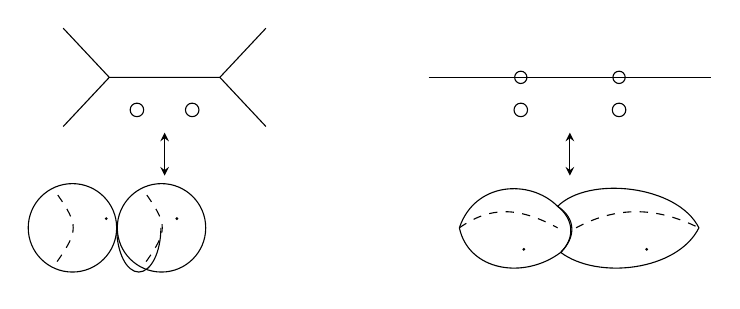
\begin{tikzpicture}[x=0.78cm,y=0.78cm,>=stealth]
 \draw (-5.8,2.05)--(-5.05,1.25)--(-3.25,1.25)--(-2.50,2.05);
 \draw (-5.8,0.45)--(-5.05,1.25) (-2.50,0.45)--(-3.25,1.25);
 \draw (-4.60,0.72) circle (0.11) (-3.70,0.72) circle (0.11);
 \draw[<->] (-4.15,0.35)--(-4.15,-0.35);
 \draw (-5.65,-1.20) circle (0.72) (-4.20,-1.20) circle (0.72);
 \draw (-4.93,-1.20) arc[start angle=180,end angle=360,x radius=0.36,y radius=0.72];
 \draw[dashed] (-5.90,-1.75) .. controls (-5.55,-1.25) and (-5.55,-1.15) .. (-5.90,-0.65);
 \draw[dashed] (-4.45,-1.75) .. controls (-4.10,-1.25) and (-4.10,-1.15) .. (-4.45,-0.65);
 \fill (-5.10,-1.05) circle (0.025) (-3.95,-1.05) circle (0.025);

 \draw (0.15,1.25)--(4.75,1.25);
 \draw (1.65,1.25) circle (0.10) (3.25,1.25) circle (0.10);
 \draw (1.65,0.72) circle (0.11) (3.25,0.72) circle (0.11);
 \draw[<->] (2.45,0.35)--(2.45,-0.35);
 \draw (0.65,-1.20) .. controls (0.90,-0.45) and (1.80,-0.40) .. (2.25,-0.85)
       .. controls (2.50,-1.05) and (2.55,-1.35) .. (2.30,-1.60)
       .. controls (1.70,-2.05) and (0.80,-1.90) .. (0.65,-1.20);
 \draw (2.30,-1.60) .. controls (2.55,-1.35) and (2.55,-1.05) .. (2.25,-0.85)
       .. controls (2.75,-0.35) and (4.20,-0.50) .. (4.55,-1.20)
       .. controls (4.20,-1.90) and (2.90,-2.05) .. (2.30,-1.60);
 \draw[dashed] (0.65,-1.20) .. controls (1.15,-0.85) and (1.60,-0.85) .. (2.25,-1.20);
 \draw[dashed] (2.55,-1.20) .. controls (3.20,-0.85) and (3.85,-0.85) .. (4.55,-1.20);
 \fill (1.70,-1.55) circle (0.025) (3.70,-1.55) circle (0.025);
\end{tikzpicture}
\caption{极小层。}
\label{fig:minimal-strata}
\end{figure}

\textbf{步骤 I：极小层。}
\stfhIndex{I204}{ji^xiao^ceng}{极小层（minimal stratum）}
设 $D$ 是定义 9.3.16 的偏序中的极小层。此时每个顶点有
$g_v=0,m_v=3$（见图\ref{fig:minimal-strata}），故每个连通相交型 $D$ 的
$\mathcal M_{g,m}^D$ 只有一个元素。回忆我们已在每个 $\Sigma_v$ 上选择凯勒度量
$h_v$，使其在 $\operatorname{Aut}(\Sigma,\boldsymbol z)$ 下不变，并在每个奇点
$x_v$ 的邻域中平坦，因而指数映射是等距映射。对每条边
$e=[v,w]\in E_T$ 及每个
$a\in T_{x_v}\Sigma_v\otimes T_{x_w}\Sigma_w\setminus\{0\}$，取唯一双全纯映射
\[
 \Phi_a:T_{x_v}\Sigma_v\setminus\{0\}
 \longrightarrow T_{x_w}\Sigma_w\setminus\{0\},
 \qquad u\otimes\Phi_a(u)=a.
\]
在 $x_v,x_w$ 的给定坐标中，正是 $\Phi_a(z)=a/z$。

再次强调，深谷--小野形变是典范的：它只依赖节点处固定的复坐标图以及截断函数
$\chi_R$ 的选择，所以不会为稳定曲线的形变描述增加参数。所得曲面记为
$\operatorname{Res}_{(\Sigma,\boldsymbol z)}(\{\alpha_e\}_{e\in E_T})$。
自同构 $\gamma$ 等距地作用于参数直和；与 $\alpha$ 和 $\gamma(\alpha)$ 对应的预稳定曲线彼此等距。
因此上述构造给出由
\[
 \frac{\bigoplus_e(T_{x_v}\Sigma_v\otimes T_{x_w}\Sigma_w)}
 {\operatorname{Aut}(\Sigma,\boldsymbol z)}
\]
中原点邻域参数化的稳定曲线族。

\begin{proposition}\label{prop:fukaya-ono-chart-minimal-stratum}
深谷--小野形变所构造的映射
\[
 \frac{\bigoplus_e(T_{x_v}\Sigma_v\otimes T_{x_w}\Sigma_w)}
 {\operatorname{Aut}(\Sigma,\boldsymbol z)}
 \longrightarrow\overline{\mathcal M}_{g,m}
\]
在 $[0]$ 的一个邻域上一一对应到其像，从而在极小层中的
$[\Sigma,\boldsymbol z]$ 处给出 $\overline{\mathcal M}_{g,m}$ 的 orbifold 图。
\end{proposition}

局部满射性的证明相当非平凡，超出本书范围；代数证明见 (DM69)，光滑证明见 (RS06)。
\begin{exercise}\label{ex:local-surjectivity-fukaya-ono-chart}
补全上述命题的证明细节，尤其是局部满射性。
\end{exercise}

orbifold 的严格讨论、$\mathcal M_{g,m}^D$ 法锥的 orbifold 结构，以及
$\overline{\mathcal M}_{g,m}$ 作为分层 orbifold 的完整描述均超出本书范围；可参见 (DM69)、(MFK94)。
这些文献把 $\overline{\mathcal M}_{g,m}$ 完整描述为德利涅--芒福德 stack。

\textbf{步骤 II：一般层。}
\stfhIndex{I038}{00-symbol-038}{$\mathcal N^D_{g,m}$}
设已对所有 $D'<D$，在 $\mathcal M_{g,m}^{D'}$ 的邻域 $\mathcal N_{g,m}^{D'}$ 上构造了每条稳定曲线的度量族，其在先前所选局部邻域的重叠处与之相容。在给定拓扑下，选择紧子集
$\mathcal K_{g,m}^D\subset\mathcal M_{g,m}^D$，使
\[
 \mathcal M_{g,m}^D\subset\mathcal K_{g,m}^D
 \cup\bigcup_{D'\le D}\mathcal N_{g,m}^{D'}.
\]
见图\ref{fig:extension-neighborhoods}。

\begin{figure}[htbp]
\centering
\setlength{\unitlength}{0.8mm}
\begin{picture}(125,38)
 \qbezier(5,8)(35,45)(62,25)
 \qbezier(62,25)(88,5)(120,28)
 \put(20,25){\circle{15}} \put(89,20){\circle{15}}
 \thicklines\qbezier(25,20)(50,35)(78,23)\thinlines
 \put(38,31){\makebox(25,5){$\mathcal K_{g,m}^D$}}
 \put(8,31){\makebox(20,5){$\mathcal N_{g,m}^{D''}$}}
 \put(82,32){\makebox(20,5){$\mathcal N_{g,m}^{D'}$}}
\end{picture}
\caption{邻域的延拓。}
\label{fig:extension-neighborhoods}
\end{figure}

有普遍纤维化
\[
 \begin{array}{ccc}
 \mathcal U_{g,m}^D&\longleftarrow&
 \displaystyle
 \frac{\bigoplus_e(T_{x_v}\Sigma_v\otimes T_{x_w}\Sigma_w)}
 {\operatorname{Aut}(\Sigma,\boldsymbol z)}\\[2mm]
 \Big\downarrow&&\\[-1mm]
 \mathcal M_{g,m}^D&&
 \end{array}
\]
它是遗忘映射
$\overline{\mathcal M}_{g,m+1}\to\overline{\mathcal M}_{g,m}$ 的限制，
并且在 $\mathcal K_{g,m}^D$ 上限制为光滑纤维化。事实上，与步骤 I 的同一构造一样，
其纤维可逐纤维地由上述参数直和模自同构群参数化。

\begin{exercise}\label{ex:universal-fibration-general-stratum}
补全这一断言的细节。
\end{exercise}

沿 $\mathcal M_{g,m}^D$ 的法向，在紧集 $\mathcal K_{g,m}^D$ 上逐纤维重复步骤 I，并延拓重叠处已有的度量。记由
$(\Sigma,\boldsymbol z)$ 表示的曲线集合为 $U_D$，以及
\[
 \Phi_D:U_D\times
 \frac{\bigoplus_{e\in E_T}(T_{x_v}\Sigma_v\otimes T_{x_w}\Sigma_w)}
 {\operatorname{Aut}(\Sigma,\boldsymbol z)}
 \longrightarrow\overline{\mathcal M}_{g,m}.
\]
所有 $\Phi_D$ 的像组成 orbifold 图册，从而给出
$\overline{\mathcal M}_{g,m}$ 的拓扑。

\begin{exercise}\label{ex:compatibility-orbifold-charts}
证明这些图在 orbifold 意义下相容。
\end{exercise}

下面的命题描述 $\mathcal M_{g,m}^D$ 在 $\overline{\mathcal M}_{g,m}$
作为分层流形（更确切地说，分层 orbifold）中的法锥结构。再一次，这一法锥的完全精确描述超出本书范围，故请读者参阅 (MFK94)。就本书的主要目的而言，只需给出精确陈述，再概述这里证明所涉及的内容。

\begin{proposition}\label{prop:universal-curve-orbifold}
$\mathcal M_{g,m}^D$ 是 orbifold，并带有纤维化
$\mathcal U_{g,m}^D\to\mathcal M_{g,m}^D$；其在
$(\Sigma,\boldsymbol z)$ 处的纤维为
$(\Sigma,\boldsymbol z)/\operatorname{Aut}(\Sigma,\boldsymbol z)$。
\end{proposition}

\begin{proof}[证明提纲]
写 $\Sigma=\bigcup_v\Sigma_v\in\mathcal M_{g,m}^D$，令 $\boldsymbol z_v$ 为
$\Sigma_v$ 上特殊点集合，$m_v=\operatorname{mark}(v)+\operatorname{sing}(v)$。
先考察位于极小层中的每一点之邻域，并逐点构造坐标图。以
$\mathcal V(\mathcal M_{g,m}^{\min})$ 表示这些图的并；它是极小层
$\mathcal M_{g,m}^{\min}$ 的开邻域。因为极小层紧，所以可用有限多个这样的乘积图覆盖它。

第二步，取下一层（记为 $D_1$）中避开
$\mathcal V(\mathcal M_{g,m}^{\min})$ 的点。这里必须注意补集
\[
 \mathcal M_{g,m}^{D_1}\setminus
 \mathcal V(\mathcal M_{g,m}^{\min})
\]
是紧的，因此同样可以用有限多个乘积图覆盖。在给定点处取该层的一个小法向切片，并把曲线每个不可约分支
$(\Sigma_v,\boldsymbol z_v)$ 的总形变写成
\[
 \mathbb C^{3g-3+m_v}/
 \operatorname{Aut}(\Sigma_v,\boldsymbol z_v).
\]
由此可选取该法向切片中的 orbifold 图。这样便得到极小层的法锥结构。完成这个初始步骤以后，第二步的图像与第一步在整个族上的版本相同；于是可在
$\mathcal M_{g,m}^{\min}$ 这族上重复第一步的过程。

接着沿对偶图集合上给定的偏序归纳进行。每到一层，都先删除已由更低层邻域覆盖的部分；剩下的是紧集，可由有限个上述局部乘积图覆盖。将所有层上得到的坐标图汇集起来，便得到
$\overline{\mathcal M}_{g,m}$ 的 orbifold 图册。这也给出命题所述普遍纤维化的局部平凡化。\footnote{译者注：原书此处仅以两句收束归纳并给出图册；“删除已覆盖部分”与“局部平凡化”两句为译者补注，内容取自源书前文的构造说明。}
\end{proof}

最后陈述此拓扑的基本定理；证明提纲与命题 9.4.26 相同。代数证明见 (DM69)，光滑论述见 (RS06)。

\begin{theorem}[德利涅--芒福德]\label{thm:deligne-mumford-compact-hausdorff}
\stfhIndex{I099}{de^li^nie^mang^fu^de}{德利涅--芒福德（Deligne–Mumford）}
赋予上述拓扑后，$\overline{\mathcal M}_{g,m}$ 是紧豪斯多夫空间。
\end{theorem}

\begin{proof}[证明提纲]
先证紧性。给定序列 $[\Sigma_i,\boldsymbol z_i]$，由定理 9.3.14，对偶图的拓扑型只有有限多个；取子列后可设它们都位于同一层
$\mathcal M_{g,m}^D$。若某个子列留在该层的紧子集内，结论成立；否则命题 9.3.19 说明标记点发生碰撞或复结构退化。完整论证需要下面的引理，其证明见 (DM69)、(RS06)。

\begin{lemma}\label{lem:degeneration-approaches-lower-stratum}
任意退化序列都有一个子列趋近某个 $D'<D$ 的层
$\mathcal M_{g,m}^{D'}$。
\end{lemma}

由命题 9.4.22，可写
\[
 (\Sigma_i,\boldsymbol z_i)=
 \operatorname{Res}_{(\Sigma_i',\boldsymbol z_i')}
 (\{\alpha'_{e,i}\}_{e\in E_T}),
\]
其中 $(\Sigma_i',\boldsymbol z_i')\in\mathcal M_{g,m}^{D'}$，且由命题 9.4.22，
$|\alpha'_{e,i}|\to0$。若 $[(\Sigma_i',\boldsymbol z_i')]$ 在
$\mathcal M_{g,m}^{D'}$ 中有收敛子列，则原序列在相应粘合坐标中也收敛，紧性即得证。若仍没有收敛子列，就对
$(\Sigma_i',\boldsymbol z_i')$ 再应用上面的论证，进入一个更低的层。每一步至少降低一次组合型；而固定 $g,m$ 时
$D$ 的型只有有限多个，所以此过程在有限步后必然停止，最终找到在
$\overline{\mathcal M}_{g,m}$ 中收敛的子列。这完成紧性的证明。\footnote{译者注：“原序列在相应粘合坐标中也收敛”与“组合型只有有限多个、过程必然停止”两句为译者对源书省略论证的显式放大；原书仅概述重复该论证直至得到收敛子列。}

再证豪斯多夫性。先注意，此处先考察稳定曲线
$(\Sigma,\boldsymbol z)$ 本身的集合而非等价类集合；它是度量空间，记相应距离函数为
$\operatorname{dist}$。用反证法，设有两个稳定曲线
$(\Sigma,\boldsymbol z)\ne(\Sigma',\boldsymbol z')$，满足
$[\Sigma,\boldsymbol z]\ne[\Sigma',\boldsymbol z']$，但存在序列
$(\Sigma_i,\boldsymbol z_i)$ 及
$\phi_i,\phi_i'\in\operatorname{Aut}(\Sigma_i,\boldsymbol z_i)$，使
\[
 \operatorname{dist}_{C^1}\bigl(\phi_i(\Sigma_i,\boldsymbol z_i),
 (\Sigma,\boldsymbol z)\bigr)\longrightarrow0,
\]
\[
 \operatorname{dist}_{C^1}\bigl(\phi_i'(\Sigma_i,\boldsymbol z_i),
 (\Sigma',\boldsymbol z')\bigr)\longrightarrow0.
\]
先考虑 $[\Sigma,\boldsymbol z]$ 与 $[\Sigma',\boldsymbol z']$ 位于同一层
$\mathcal M_{g,m}^D$ 的情形。若两个极限与序列也在同一层，可把序列表示在同一节点曲面上，令
$\psi_i=\phi_i'\circ\phi_i^{-1}:\Sigma\to\Sigma'$。

更明确地，先只把 $[\Sigma_i,\boldsymbol z_i]$ 看作等价类，而暂不固定代表。\footnote{译者注：本句为译者补注，用以澄清代表元的选取方式；原书无此句。}在同层情形，取子列后可用一个固定的节点曲面
$\Sigma$ 表示它们，使
\[
 \phi_i((\Sigma_i,j_i),\boldsymbol z_i)
 =((\Sigma,\widetilde j_i),\boldsymbol x_i),
 \qquad (\widetilde j_i,\boldsymbol x_i)\to(j,\boldsymbol z).
\]
同样有
\[
 \phi_i'((\Sigma_i,j_i),\boldsymbol z_i)
 =((\Sigma',\widetilde j_i'),\boldsymbol x_i'),
 \qquad (\widetilde j_i',\boldsymbol x_i')\to(j',\boldsymbol z').
\]
于是 $\psi_i=\phi_i'\circ\phi_i^{-1}$ 满足
$(\psi_i)_*\widetilde j_i\to\widetilde j_i'$ 且
$\psi_i(\boldsymbol x_i)\to\boldsymbol x_i'$；它是
$(\widetilde j_i,\widetilde j_i')$-全纯的。

\begin{lemma}\label{lem:equicontinuity-biholomorphisms-stable-curves}
序列 $\psi_i$ 等度连续，因而有一个在 $C^\infty$-拓扑中收敛的子列。
\end{lemma}

\begin{proof}
只需在每个不可约分支上证明 $|d\psi_i|_{C^1}<C$。否则，依第 9.2 节的冒泡论证可产生非恒定
$(j,j')$-全纯球面 $v:S^2\to\Sigma'$，且 $\int v^*\omega'>0$。若
$\operatorname{genus}(\Sigma')\ge1$，则 $\pi_2(\Sigma')=0$，矛盾。若亏格为零，则源、靶都可视为
$\mathbb{CP}^1$，各 $\psi_i\in PSL(2,\mathbb C)$。稳定性给出
$\#(\boldsymbol z_i)=\#(\boldsymbol z_i')\ge3$。利用
$(\widetilde j_i',\boldsymbol x_i')\to(j',\boldsymbol z')$ 与
$(\widetilde j_i,\boldsymbol x_i)\to(j,\boldsymbol z)$，并对源、靶施以自同构，可令其中三点分别为
$0,1,\infty$，且有统一的分离常数
\[
 \operatorname{dist}(\psi_i(0),\psi_i(1)),
 \operatorname{dist}(\psi_i(0),\psi_i(1)),
 \operatorname{dist}(\psi_i(0),\psi_i(1))\ge\delta>0.
\]
这说明 $\{\psi_i\}\subset PSL(2,\mathbb C)$ 预紧，从而有收敛到
$(\mathbb{CP}^1,\boldsymbol z)$ 与
$(\mathbb{CP}^1,\boldsymbol z')$ 之间同构的子列。高阶收敛由主估计定理 8.3.5 给出。
\end{proof}

引理表明 $\psi_i$ 的子列趋于双全纯映射
$\psi:(\Sigma,\boldsymbol z)\to(\Sigma',\boldsymbol z')$，这与二极限非同构的反设矛盾。

再设两个极限位于同一层 $D$，而序列位于另一层 $D'$。利用解节点图，可以写
\[
 \phi_i((\Sigma_i,j_i),\boldsymbol z_i)
 =\operatorname{Res}_{(\Sigma,\boldsymbol z)}(\alpha_i),
 \qquad
 \phi_i'((\Sigma_i,j_i),\boldsymbol z_i)
 =\operatorname{Res}_{(\Sigma',\boldsymbol z')}(\alpha_i'),
\]
其中 $|\alpha_i|,|\alpha_i'|\to0$。取子列后可令
$\Sigma_i=\Sigma''$ 对所有 $i$ 成立。于是，当
$|\alpha_i|,|\alpha_i'|\to0$ 时，映射
$\phi_i'\circ\phi_i^{-1}:\Sigma''\to\Sigma''$ 给出一个双全纯映射
$\psi:(\Sigma,\boldsymbol z)\to(\Sigma',\boldsymbol z')$，使
$\psi(\Sigma,\boldsymbol z)=(\Sigma',\boldsymbol z')$ 且
$|\alpha_i-\alpha_i'|\to0$。这再次同
$[\Sigma,\boldsymbol z]\ne[\Sigma',\boldsymbol z']$ 矛盾。

最后还剩 $[\Sigma,\boldsymbol z]$ 与 $[\Sigma',\boldsymbol z']$ 位于两个不同层的情形。
这一情形甚至比前一种更容易处理，留给读者。

\begin{exercise}\label{ex:hausdorff-different-strata}
补全上述证明中 $[\Sigma,\boldsymbol z]$ 与
$[\Sigma',\boldsymbol z']$ 位于不同层时的细节。
\end{exercise}
\end{proof}
